\begin{figure}[H]
    \centering
    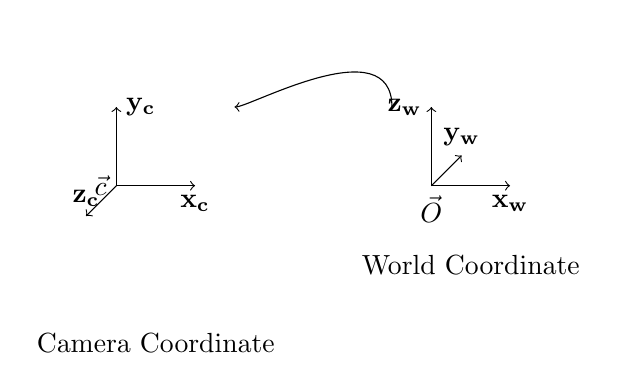
\begin{tikzpicture}[->]
        \begin{scope}[xshift=3.5cm]
            \draw (0,0,0) -- (xyz cs:x=1)node[below]{$\bf{x}_w$};
            \draw (0,0,0) -- (xyz cs:y=1)node[left]{$\bf{z}_w$};
            \draw (0,0,0) -- (xyz cs:z=-1)node[above]{$\bf{y}_w$};
            \node (O) at (0,0,0) [below] {$\vec{O}$};
        \end{scope}
        \draw[->] (3,1) .. controls +(up:1cm) and +(right:0.2cm) .. (1, 1);
        \begin{scope}[xshift=-0.5cm]
            \draw (0,0,0) -- (xyz cs:x=1)node[below]{$\bf{x}_c$};
            \draw (0,0,0) -- (xyz cs:y=1)node[right]{$\bf{y}_c$};
            \draw (0,0,0) -- (xyz cs:z=1)node[above]{$\bf{z}_c$};
            \node (P) at (0,0,0) [left] {$\vec{c}$};
        \end{scope}
        \node (A) at (0, -2) {Camera Coordinate};
        \node (B) at (4, -1) {World Coordinate};
    \end{tikzpicture}
    \caption{FlipZ Camera Model}
    \label{fig:flip_z_camera}
\end{figure}


如图\ref{fig:flip_z_camera}所示,一个正常的右手系世界坐标系$\bf{x_w,y_w,z_w}$和原点$\bf{O}$下,
相机视角的局部坐标系$\bf{x_c,y_c,z_c}$和相机原点在世界坐标系下的坐标 $\bf{p}_c$

$$\left[\begin{matrix} 
    \vec{x}_c \\ \vec{y}_c \\ \vec{z}_c 
\end{matrix}\right]=
\left[\begin{matrix} 
    x_{c0} & x_{c1} & x_{c2} \\ 
    y_{c0} & y_{c1} & y_{c2} \\ 
    z_{c0} & z_{c1} & z_{c2} 
\end{matrix}\right]
\left[\begin{matrix} 
    \vec{x} \\ \vec{y} \\ \vec{z} 
\end{matrix}\right]=
R\left[\begin{matrix} 
    \vec{x} \\ \vec{y} \\ \vec{z} 
\end{matrix}\right]$$

在相机确定之后,任意一个世界坐标$(p_{wx},p_{wy},p_{wz})$都可以经过一个旋转
和一个平移变换到相机坐标系$(p_{cx},p_{cy},p_{cz})$之中,我们不妨引入齐次坐标的概念

来确定一个$4\times 4$的变换矩阵$\bf{M}$,使得

$[p_{cx},p_{cy},p_{cz},1]=[p_{wx},p_{wy},p_{wz},1]\bf{M}$

并且可以推导出$\bf{M}$的表达式

$$[p_{wx},p_{wy},p_{wz},1]
\left[\begin{matrix} 
    x_{c0} & y_{c0} & z_{c0} & 0 \\ 
    x_{c1} & y_{c1} & z_{c1} & 0 \\ 
    x_{c2} & y_{c2} & z_{c2} & 0 \\ 
    -\vec{c}\cdot\vec{x}_c &-\vec{c}\cdot\vec{y}_c &-\vec{c}\cdot\vec{z}_c & 1 
\end{matrix}\right]=[p_{cx},p_{cy},p_{cz}, 1]$$


这里的M被称为View Matrix视角矩阵。它的作用就是把一个世界坐标系下的点变换到相机局部坐标系(NDC)下。
GLM的默认配置就是flipz的,所以可以直接实现
